% Options for packages loaded elsewhere
\PassOptionsToPackage{unicode}{hyperref}
\PassOptionsToPackage{hyphens}{url}
%
\documentclass[
  ignorenonframetext,
]{beamer}
\usepackage{pgfpages}
\setbeamertemplate{caption}[numbered]
\setbeamertemplate{caption label separator}{: }
\setbeamercolor{caption name}{fg=normal text.fg}
\beamertemplatenavigationsymbolsempty
% Prevent slide breaks in the middle of a paragraph
\widowpenalties 1 10000
\raggedbottom
\setbeamertemplate{part page}{
  \centering
  \begin{beamercolorbox}[sep=16pt,center]{part title}
    \usebeamerfont{part title}\insertpart\par
  \end{beamercolorbox}
}
\setbeamertemplate{section page}{
  \centering
  \begin{beamercolorbox}[sep=12pt,center]{part title}
    \usebeamerfont{section title}\insertsection\par
  \end{beamercolorbox}
}
\setbeamertemplate{subsection page}{
  \centering
  \begin{beamercolorbox}[sep=8pt,center]{part title}
    \usebeamerfont{subsection title}\insertsubsection\par
  \end{beamercolorbox}
}
\AtBeginPart{
  \frame{\partpage}
}
\AtBeginSection{
  \ifbibliography
  \else
    \frame{\sectionpage}
  \fi
}
\AtBeginSubsection{
  \frame{\subsectionpage}
}
\usepackage{lmodern}
\usepackage{amssymb,amsmath}
\usepackage{ifxetex,ifluatex}
\ifnum 0\ifxetex 1\fi\ifluatex 1\fi=0 % if pdftex
  \usepackage[T1]{fontenc}
  \usepackage[utf8]{inputenc}
  \usepackage{textcomp} % provide euro and other symbols
\else % if luatex or xetex
  \usepackage{unicode-math}
  \defaultfontfeatures{Scale=MatchLowercase}
  \defaultfontfeatures[\rmfamily]{Ligatures=TeX,Scale=1}
\fi
% Use upquote if available, for straight quotes in verbatim environments
\IfFileExists{upquote.sty}{\usepackage{upquote}}{}
\IfFileExists{microtype.sty}{% use microtype if available
  \usepackage[]{microtype}
  \UseMicrotypeSet[protrusion]{basicmath} % disable protrusion for tt fonts
}{}
\makeatletter
\@ifundefined{KOMAClassName}{% if non-KOMA class
  \IfFileExists{parskip.sty}{%
    \usepackage{parskip}
  }{% else
    \setlength{\parindent}{0pt}
    \setlength{\parskip}{6pt plus 2pt minus 1pt}}
}{% if KOMA class
  \KOMAoptions{parskip=half}}
\makeatother
\usepackage{xcolor}
\IfFileExists{xurl.sty}{\usepackage{xurl}}{} % add URL line breaks if available
\IfFileExists{bookmark.sty}{\usepackage{bookmark}}{\usepackage{hyperref}}
\hypersetup{
  pdftitle={R\^{}4HO: R for Water Professionals: Session 2},
  pdfauthor={Dr Peter Prevos},
  hidelinks,
  pdfcreator={LaTeX via pandoc}}
\urlstyle{same} % disable monospaced font for URLs
\newif\ifbibliography
\usepackage{color}
\usepackage{fancyvrb}
\newcommand{\VerbBar}{|}
\newcommand{\VERB}{\Verb[commandchars=\\\{\}]}
\DefineVerbatimEnvironment{Highlighting}{Verbatim}{commandchars=\\\{\}}
% Add ',fontsize=\small' for more characters per line
\usepackage{framed}
\definecolor{shadecolor}{RGB}{248,248,248}
\newenvironment{Shaded}{\begin{snugshade}}{\end{snugshade}}
\newcommand{\AlertTok}[1]{\textcolor[rgb]{0.94,0.16,0.16}{#1}}
\newcommand{\AnnotationTok}[1]{\textcolor[rgb]{0.56,0.35,0.01}{\textbf{\textit{#1}}}}
\newcommand{\AttributeTok}[1]{\textcolor[rgb]{0.77,0.63,0.00}{#1}}
\newcommand{\BaseNTok}[1]{\textcolor[rgb]{0.00,0.00,0.81}{#1}}
\newcommand{\BuiltInTok}[1]{#1}
\newcommand{\CharTok}[1]{\textcolor[rgb]{0.31,0.60,0.02}{#1}}
\newcommand{\CommentTok}[1]{\textcolor[rgb]{0.56,0.35,0.01}{\textit{#1}}}
\newcommand{\CommentVarTok}[1]{\textcolor[rgb]{0.56,0.35,0.01}{\textbf{\textit{#1}}}}
\newcommand{\ConstantTok}[1]{\textcolor[rgb]{0.00,0.00,0.00}{#1}}
\newcommand{\ControlFlowTok}[1]{\textcolor[rgb]{0.13,0.29,0.53}{\textbf{#1}}}
\newcommand{\DataTypeTok}[1]{\textcolor[rgb]{0.13,0.29,0.53}{#1}}
\newcommand{\DecValTok}[1]{\textcolor[rgb]{0.00,0.00,0.81}{#1}}
\newcommand{\DocumentationTok}[1]{\textcolor[rgb]{0.56,0.35,0.01}{\textbf{\textit{#1}}}}
\newcommand{\ErrorTok}[1]{\textcolor[rgb]{0.64,0.00,0.00}{\textbf{#1}}}
\newcommand{\ExtensionTok}[1]{#1}
\newcommand{\FloatTok}[1]{\textcolor[rgb]{0.00,0.00,0.81}{#1}}
\newcommand{\FunctionTok}[1]{\textcolor[rgb]{0.00,0.00,0.00}{#1}}
\newcommand{\ImportTok}[1]{#1}
\newcommand{\InformationTok}[1]{\textcolor[rgb]{0.56,0.35,0.01}{\textbf{\textit{#1}}}}
\newcommand{\KeywordTok}[1]{\textcolor[rgb]{0.13,0.29,0.53}{\textbf{#1}}}
\newcommand{\NormalTok}[1]{#1}
\newcommand{\OperatorTok}[1]{\textcolor[rgb]{0.81,0.36,0.00}{\textbf{#1}}}
\newcommand{\OtherTok}[1]{\textcolor[rgb]{0.56,0.35,0.01}{#1}}
\newcommand{\PreprocessorTok}[1]{\textcolor[rgb]{0.56,0.35,0.01}{\textit{#1}}}
\newcommand{\RegionMarkerTok}[1]{#1}
\newcommand{\SpecialCharTok}[1]{\textcolor[rgb]{0.00,0.00,0.00}{#1}}
\newcommand{\SpecialStringTok}[1]{\textcolor[rgb]{0.31,0.60,0.02}{#1}}
\newcommand{\StringTok}[1]{\textcolor[rgb]{0.31,0.60,0.02}{#1}}
\newcommand{\VariableTok}[1]{\textcolor[rgb]{0.00,0.00,0.00}{#1}}
\newcommand{\VerbatimStringTok}[1]{\textcolor[rgb]{0.31,0.60,0.02}{#1}}
\newcommand{\WarningTok}[1]{\textcolor[rgb]{0.56,0.35,0.01}{\textbf{\textit{#1}}}}
\usepackage{graphicx}
\makeatletter
\def\maxwidth{\ifdim\Gin@nat@width>\linewidth\linewidth\else\Gin@nat@width\fi}
\def\maxheight{\ifdim\Gin@nat@height>\textheight\textheight\else\Gin@nat@height\fi}
\makeatother
% Scale images if necessary, so that they will not overflow the page
% margins by default, and it is still possible to overwrite the defaults
% using explicit options in \includegraphics[width, height, ...]{}
\setkeys{Gin}{width=\maxwidth,height=\maxheight,keepaspectratio}
% Set default figure placement to htbp
\makeatletter
\def\fps@figure{htbp}
\makeatother
\setlength{\emergencystretch}{3em} % prevent overfull lines
\providecommand{\tightlist}{%
  \setlength{\itemsep}{0pt}\setlength{\parskip}{0pt}}
\setcounter{secnumdepth}{-\maxdimen} % remove section numbering

\title{\(R^4\)H\textsubscript{2}O: R for Water Professionals: Session 2}
\author{Dr Peter Prevos}
\date{}

\begin{document}
\frame{\titlepage}

\begin{frame}{Session 2 Program}
\protect\hypertarget{session-2-program}{}
\begin{columns}[T]
\begin{column}{0.48\textwidth}
\begin{itemize}
\tightlist
\item
  Recap
\item
  Data Visualisation
\item
  Creating Data Products
\end{itemize}
\end{column}

\begin{column}{0.48\textwidth}
\begin{figure}
\centering
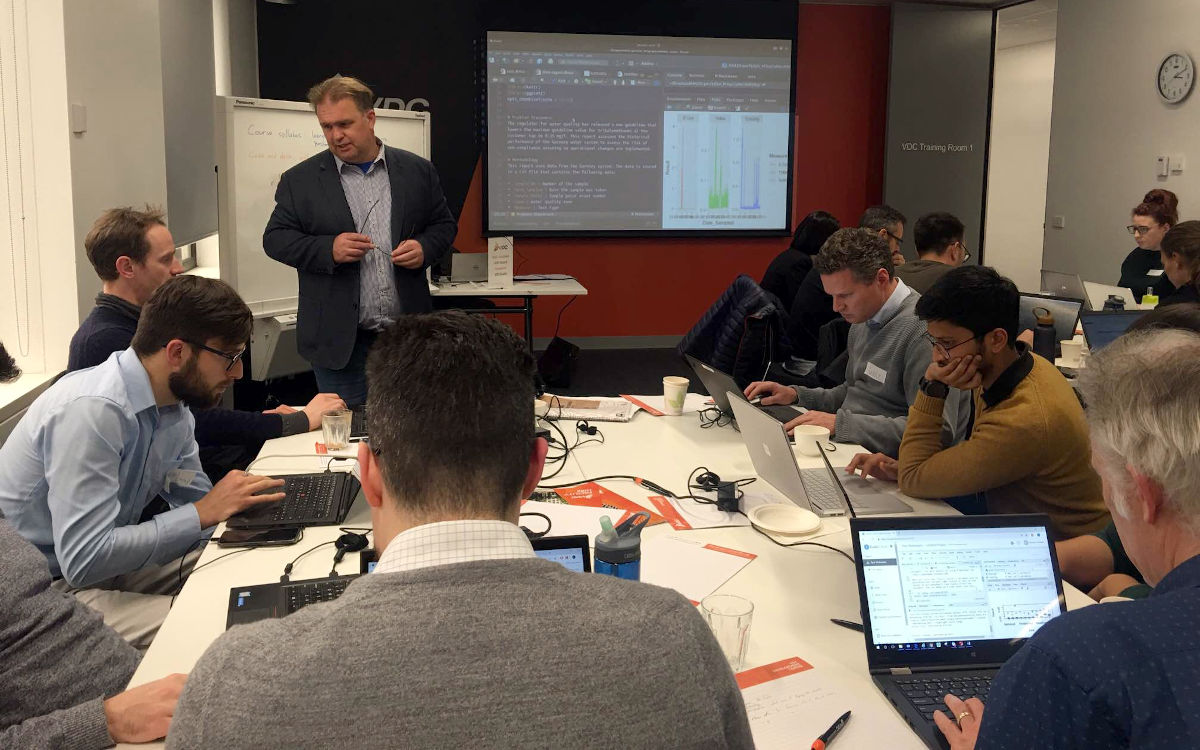
\includegraphics{../manuscript/resources/01_introduction/2019_workshop_melbourne.jpg}
\caption{R for Water Professionals workshop (Melbourne, 2019).}
\end{figure}
\end{column}
\end{columns}
\end{frame}

\begin{frame}[fragile]{R Basics}
\protect\hypertarget{r-basics}{}
Which of these expressions calculates the flow in cubic meters per
second for all heights (\texttt{h}) between 50mm and 500mm? Type them
into the console to try each option and inspect the output.

\begin{Shaded}
\begin{Highlighting}[]
\NormalTok{Cd \textless{}{-}}\StringTok{ }\FloatTok{0.6}
\NormalTok{g \textless{}{-}}\StringTok{ }\FloatTok{9.81}
\NormalTok{b \textless{}{-}}\StringTok{ }\FloatTok{0.6}

\NormalTok{(}\DecValTok{2}\OperatorTok{/}\DecValTok{3}\NormalTok{) }\OperatorTok{*}\StringTok{ }\NormalTok{Cd }\OperatorTok{*}\StringTok{ }\KeywordTok{sqrt}\NormalTok{(}\DecValTok{2} \OperatorTok{*}\StringTok{ }\FloatTok{9.81}\NormalTok{) }\OperatorTok{*}\StringTok{ }\NormalTok{b }\OperatorTok{*}\StringTok{ }\NormalTok{(}\FloatTok{0.05}\OperatorTok{:}\FloatTok{0.50}\NormalTok{)}\OperatorTok{\^{}}\NormalTok{(}\DecValTok{3}\OperatorTok{/}\DecValTok{2}\NormalTok{)}

\NormalTok{(}\DecValTok{2}\OperatorTok{/}\DecValTok{3}\NormalTok{) }\OperatorTok{*}\StringTok{ }\NormalTok{Cd }\OperatorTok{*}\StringTok{ }\KeywordTok{sqrt}\NormalTok{(}\DecValTok{2} \OperatorTok{*}\StringTok{ }\FloatTok{9.81}\NormalTok{) }\OperatorTok{*}\StringTok{ }\NormalTok{b }\OperatorTok{*}\StringTok{ }\NormalTok{((}\DecValTok{50}\OperatorTok{:}\DecValTok{500}\NormalTok{)}\OperatorTok{/}\DecValTok{1000}\NormalTok{)}\OperatorTok{\^{}}\NormalTok{(}\DecValTok{3}\OperatorTok{/}\DecValTok{2}\NormalTok{)}
\end{Highlighting}
\end{Shaded}

Or, repeat the formula for each value of \texttt{h}.

\begin{Shaded}
\begin{Highlighting}[]
\NormalTok{h \textless{}{-}}\StringTok{ }\KeywordTok{seq}\NormalTok{(.}\DecValTok{05}\NormalTok{, }\FloatTok{.5}\NormalTok{, }\FloatTok{.01}\NormalTok{)}
\end{Highlighting}
\end{Shaded}
\end{frame}

\begin{frame}[fragile]{Loading and Exploring Data}
\protect\hypertarget{loading-and-exploring-data}{}
\begin{Shaded}
\begin{Highlighting}[]
\KeywordTok{library}\NormalTok{(tidyverse)}
\NormalTok{gormsey \textless{}{-}}\StringTok{ }\KeywordTok{read\_csv}\NormalTok{(}\StringTok{"casestudy1/gormsey.csv"}\NormalTok{)}

\NormalTok{gormsey\_tt \textless{}{-}}\StringTok{ }\KeywordTok{filter}\NormalTok{(gormsey, Measure }\OperatorTok{==}\StringTok{ "Turbidity"} \OperatorTok{|}\StringTok{ }\NormalTok{Measure }\OperatorTok{==}\StringTok{ "THM"}\NormalTok{)}

\KeywordTok{count}\NormalTok{(gormsey\_tt, Measure)}

\NormalTok{gormsey\_grouped \textless{}{-}}\StringTok{ }\KeywordTok{group\_by}\NormalTok{(gormsey\_tt, Measure, Town)}
\KeywordTok{summarise}\NormalTok{(gormsey\_grouped, }\DataTypeTok{p95 =} \KeywordTok{quantile}\NormalTok{(Result, }\FloatTok{0.99}\NormalTok{))}
\end{Highlighting}
\end{Shaded}
\end{frame}

\begin{frame}{Data Visualisation}
\protect\hypertarget{data-visualisation}{}
\begin{columns}[T]
\begin{column}{0.48\textwidth}
\begin{figure}
\centering
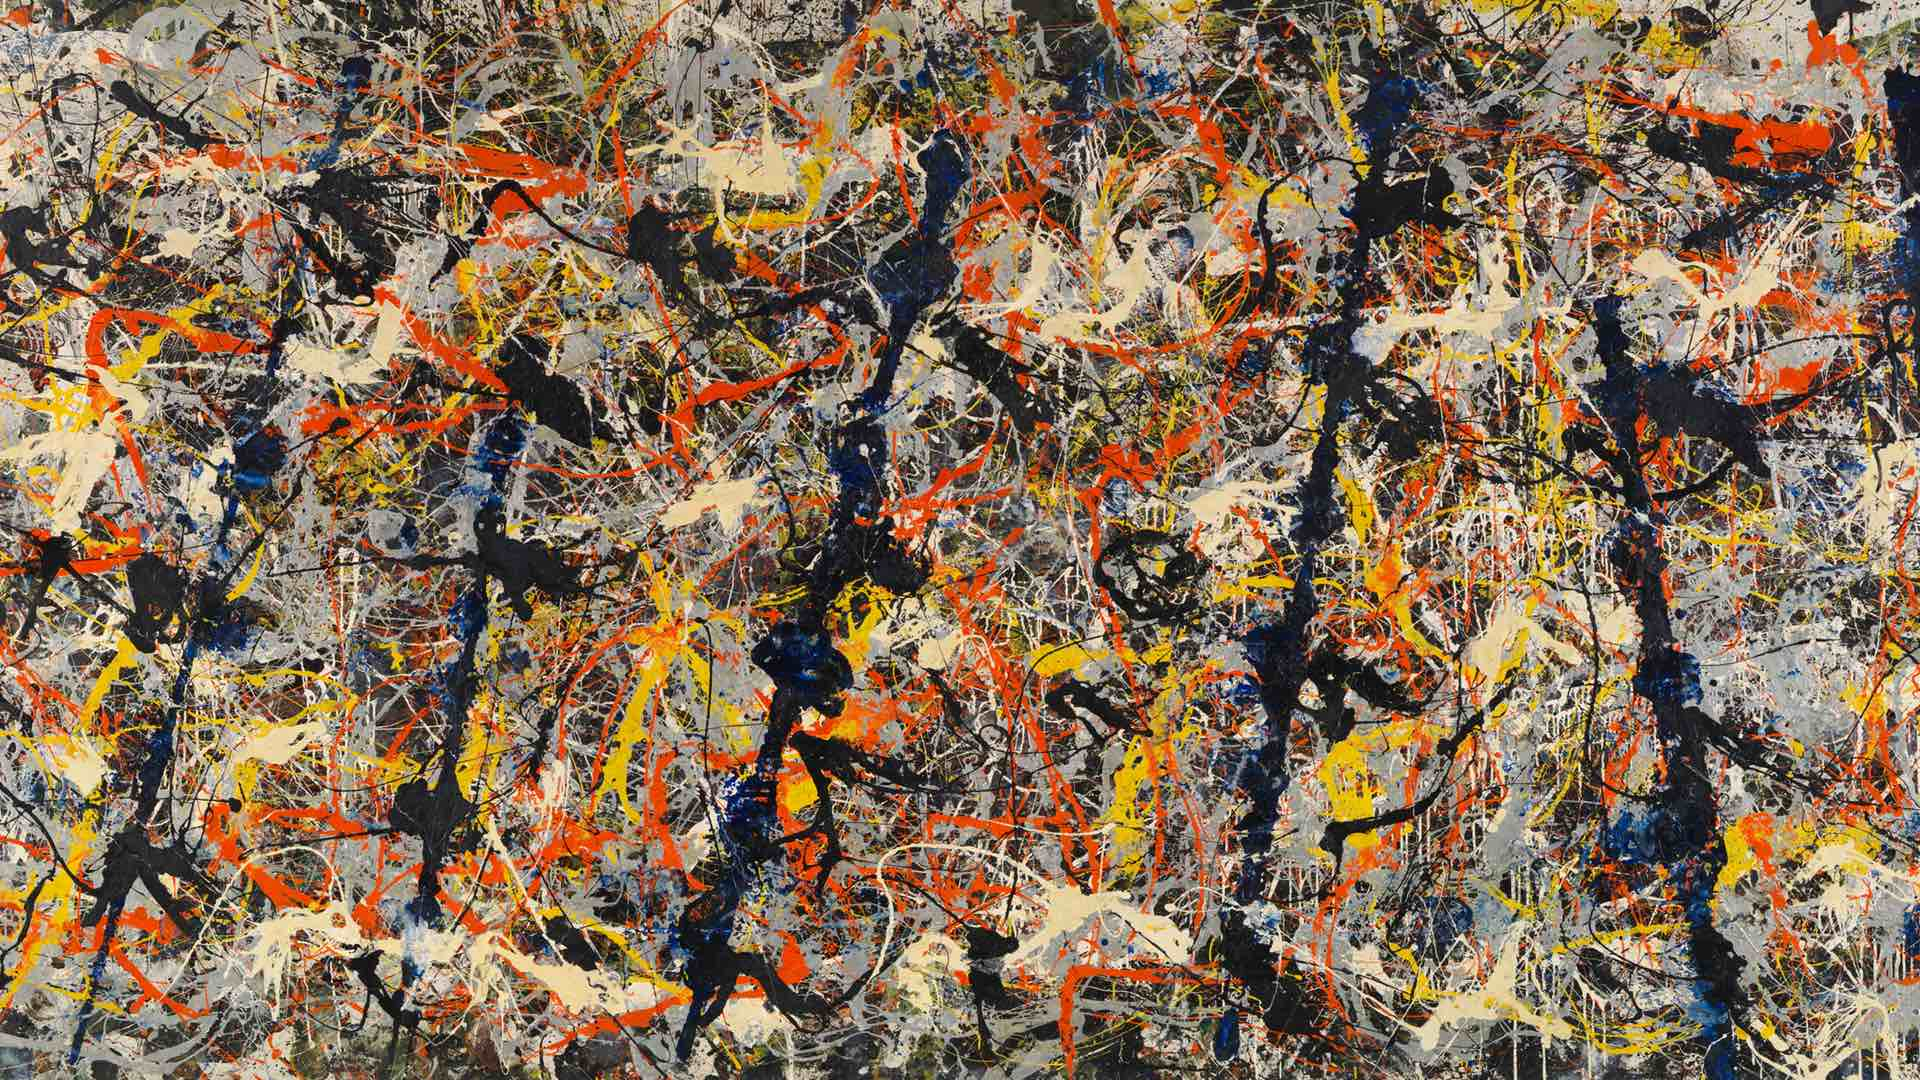
\includegraphics{../manuscript/resources/06_visualisation/bluepoles.jpg}
\caption{Jackson Pollock, \emph{Blue Poles} (1973).}
\end{figure}
\end{column}

\begin{column}{0.48\textwidth}
\begin{figure}
\centering
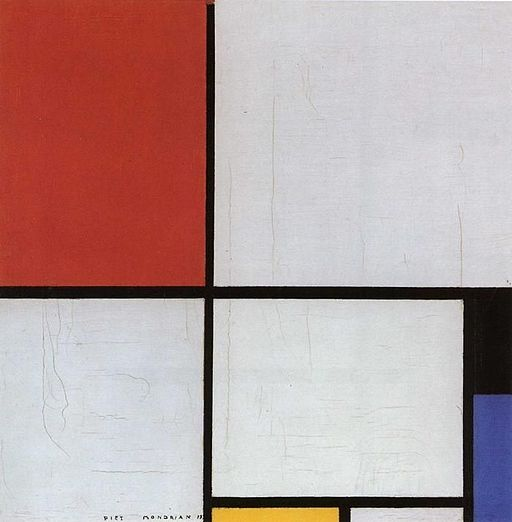
\includegraphics{../manuscript/resources/06_visualisation/mondrian.jpg}
\caption{Piet Mondrian, \emph{Composition in Red, Yellow and Blue}
(1928)}
\end{figure}
\end{column}
\end{columns}
\end{frame}

\begin{frame}{Data-to-Pixel Ratio}
\protect\hypertarget{data-to-pixel-ratio}{}
\begin{figure}
\centering
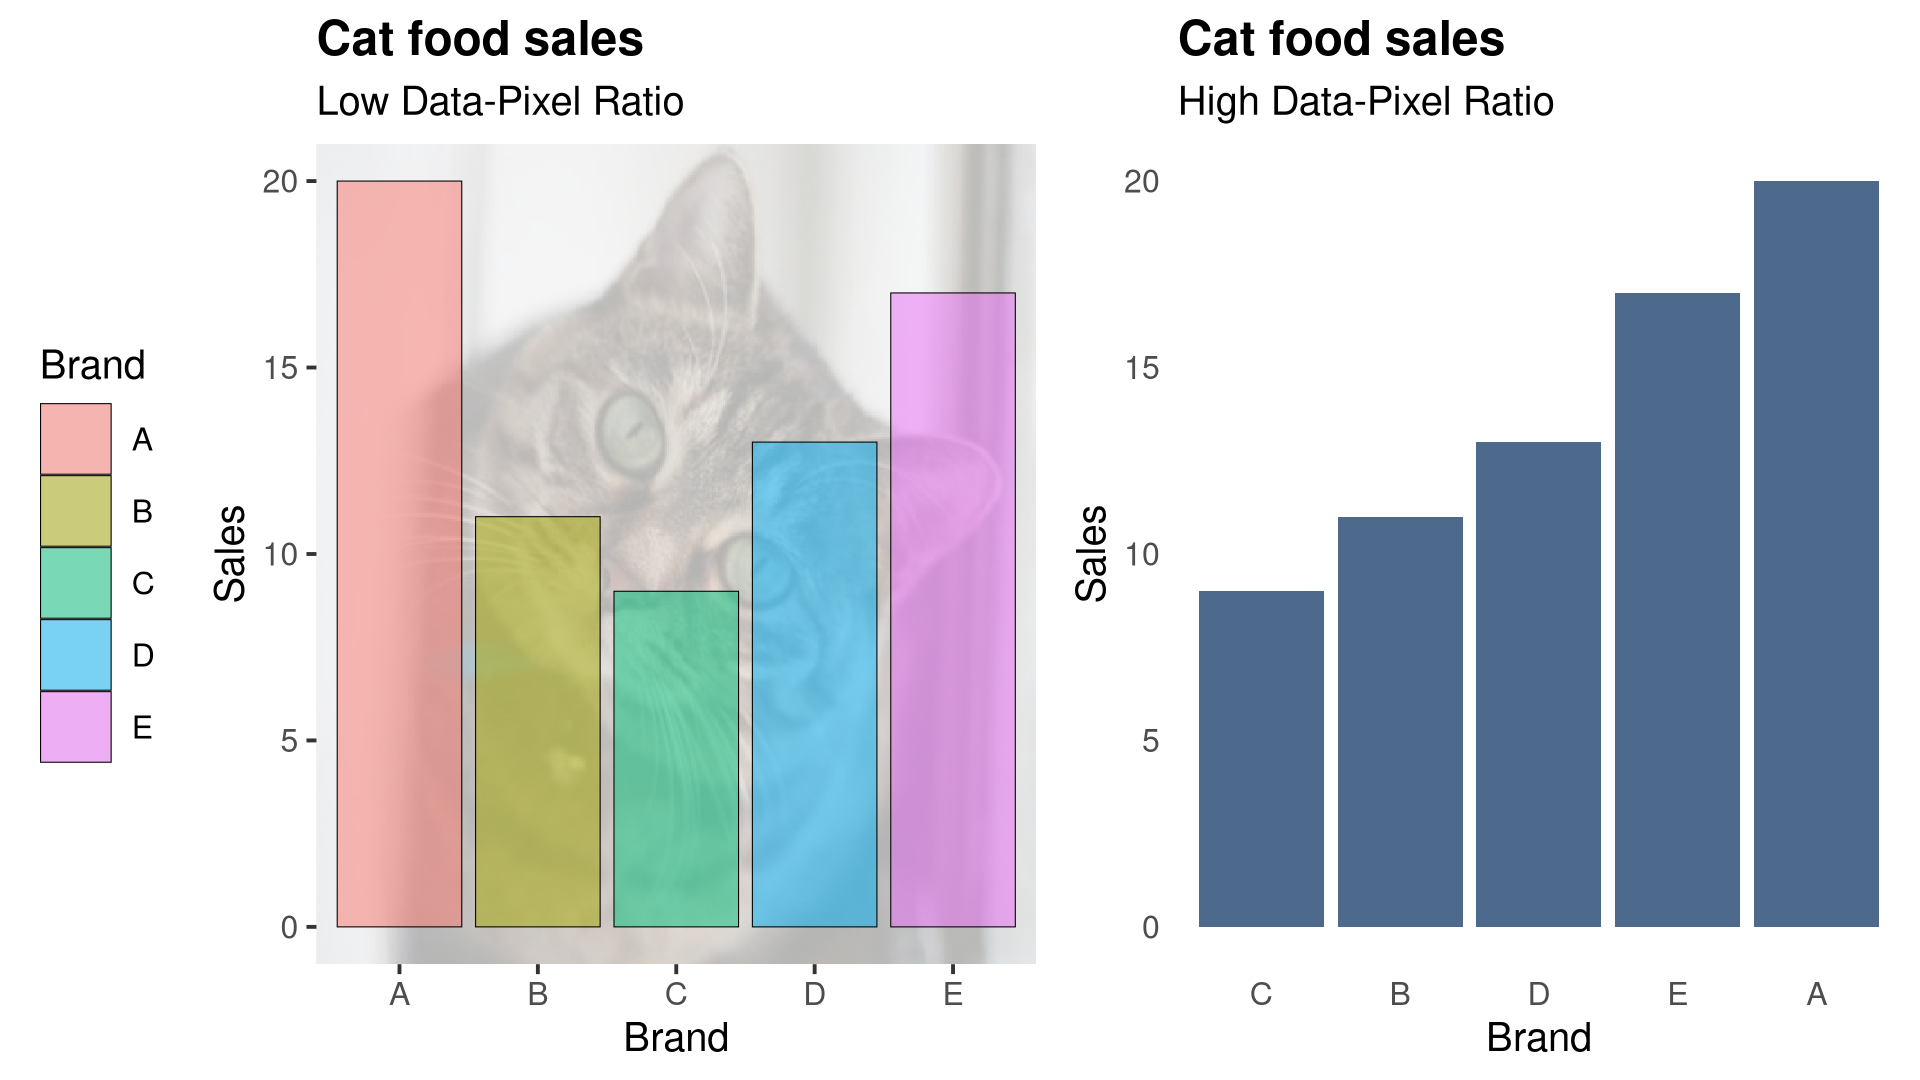
\includegraphics{../manuscript/resources/06_visualisation/data-pixel-ratio.png}
\caption{Maximise the data to pixel ratio for aesthetic visualisations.}
\end{figure}
\end{frame}

\begin{frame}{Chart Chooser}
\protect\hypertarget{chart-chooser}{}
\begin{figure}
\centering
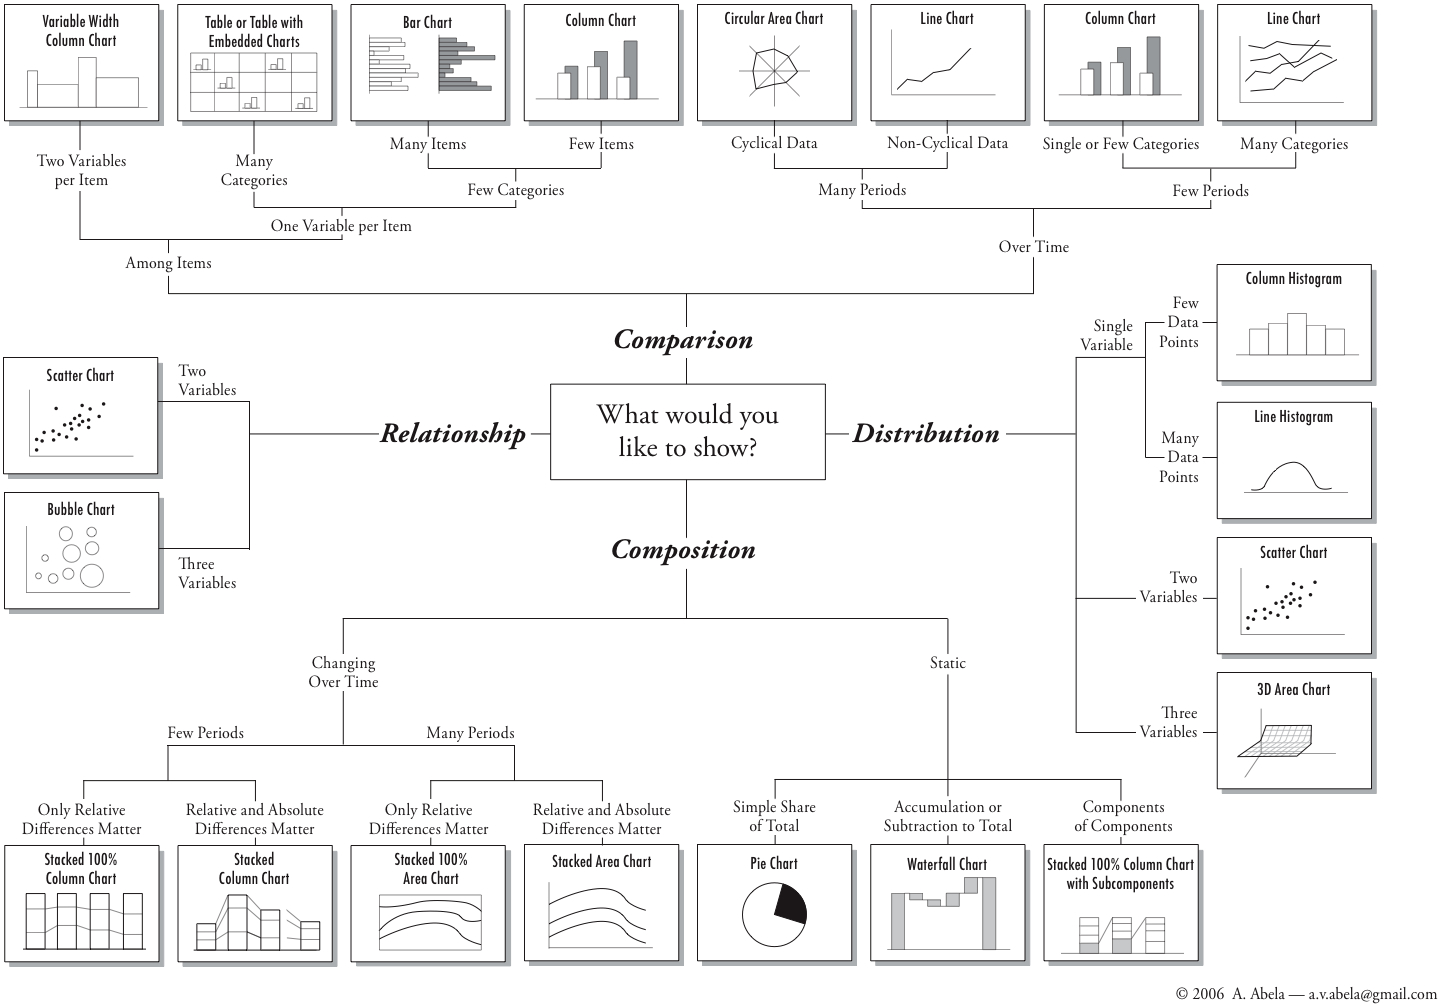
\includegraphics{images/chart_chooser.png}
\caption{Chart suggestions by Andrew Abela.}
\end{figure}
\end{frame}

\begin{frame}{Use Colours Sparingly}
\protect\hypertarget{use-colours-sparingly}{}
\begin{figure}
\centering
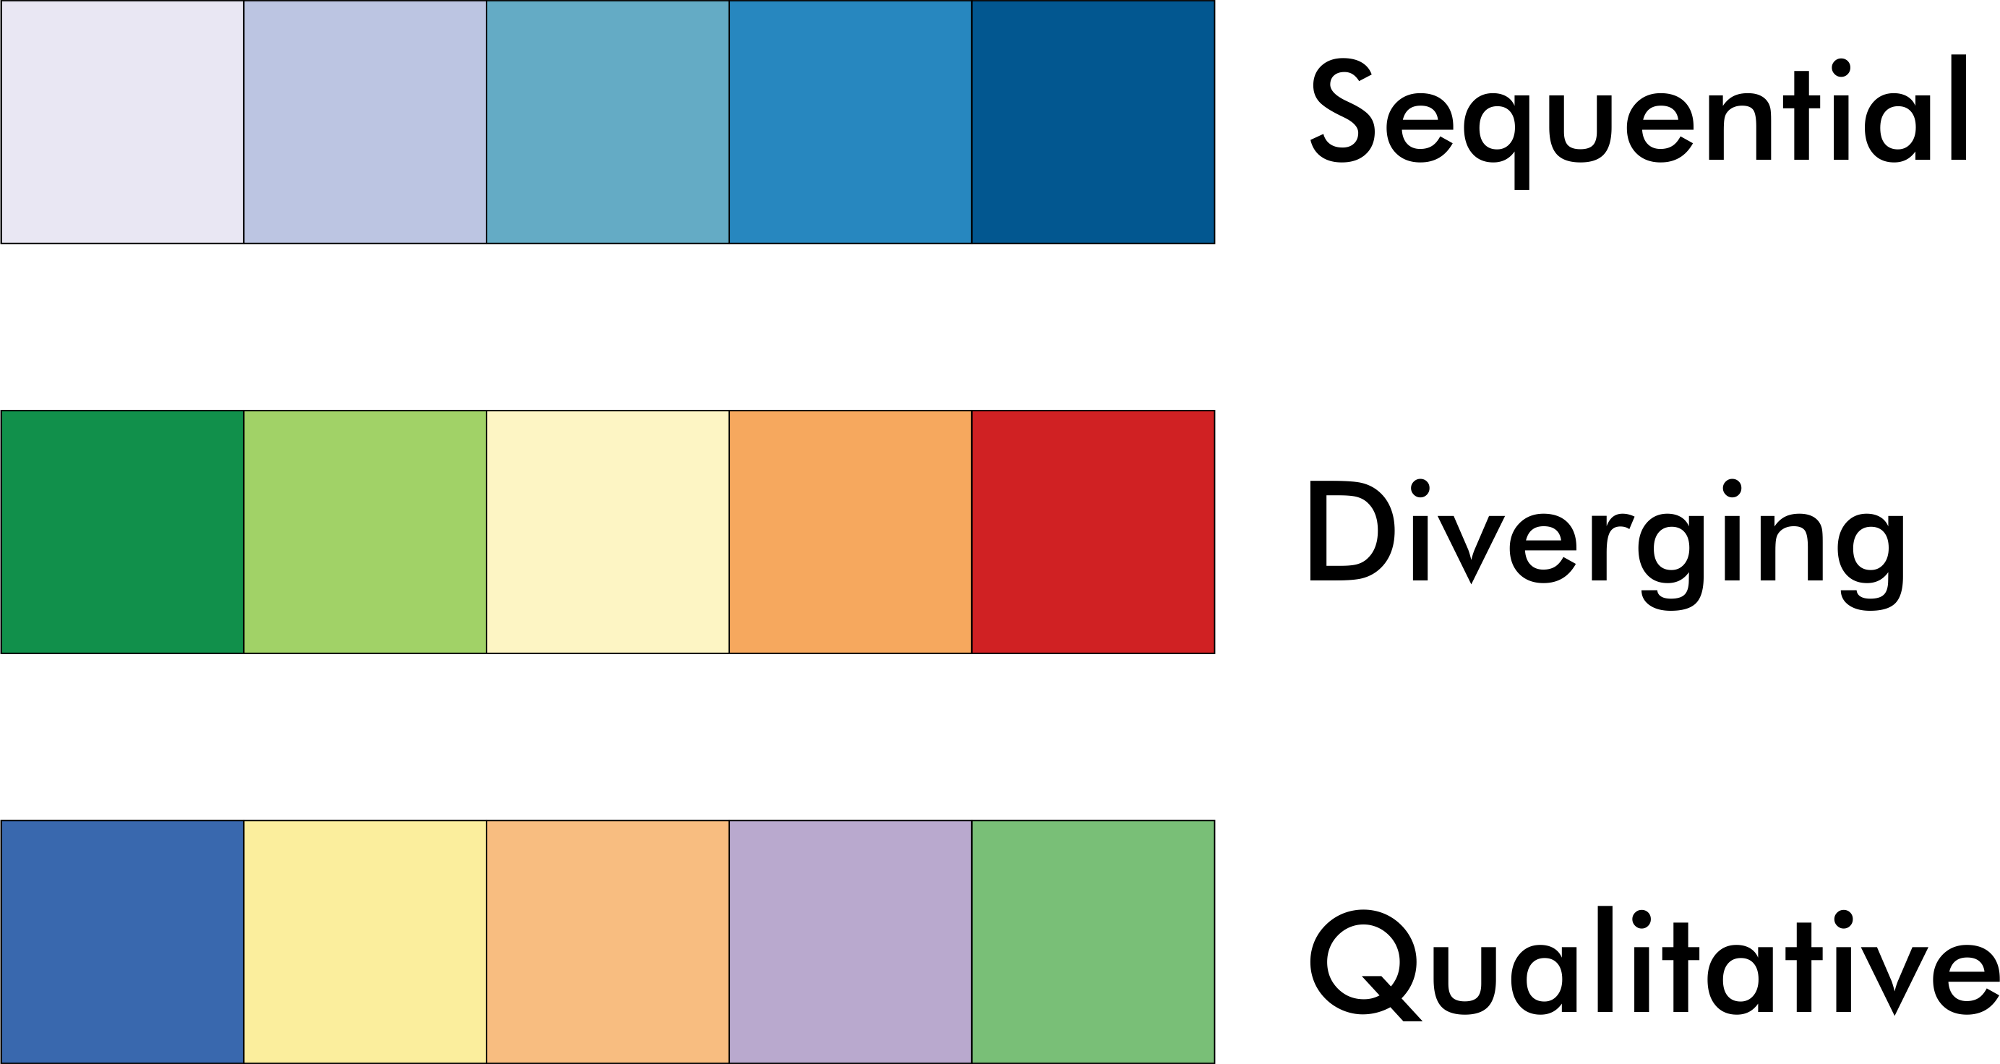
\includegraphics{../manuscript/resources/06_visualisation/ColorBrewer.png}
\caption{Types of colour pallets. Go to \url{colorbrewer2.org} for
details.}
\end{figure}
\end{frame}

\begin{frame}[fragile]{ggplot2}
\protect\hypertarget{ggplot2}{}
\begin{columns}[T]
\begin{column}{0.48\textwidth}
\begin{itemize}
\tightlist
\item
  System for creating graphics, based on \emph{The Grammar of Graphics}.
\item
  Go to \href{https://ggplot2.tidyverse.org/}{ggplot2.tidyverse.org} for
  documentation.
\item
  Included in the Tidyverse. You can call it separately with:
\end{itemize}

\begin{Shaded}
\begin{Highlighting}[]
\KeywordTok{library}\NormalTok{(ggplot2)}
\end{Highlighting}
\end{Shaded}
\end{column}

\begin{column}{0.48\textwidth}

\includegraphics{images/ggplot2.png}
\end{column}
\end{columns}
\end{frame}

\begin{frame}{Grammar of Graphics}
\protect\hypertarget{grammar-of-graphics}{}
\begin{columns}[T]
\begin{column}{0.48\textwidth}
\begin{figure}
\centering

\includegraphics{../manuscript/resources/06_visualisation/grammar_of_graphics.jpg}
\caption{Leland Wilkinson, \emph{Grammar of Graphics} (2005).}
\end{figure}
\end{column}

\begin{column}{0.48\textwidth}
\begin{figure}
\centering
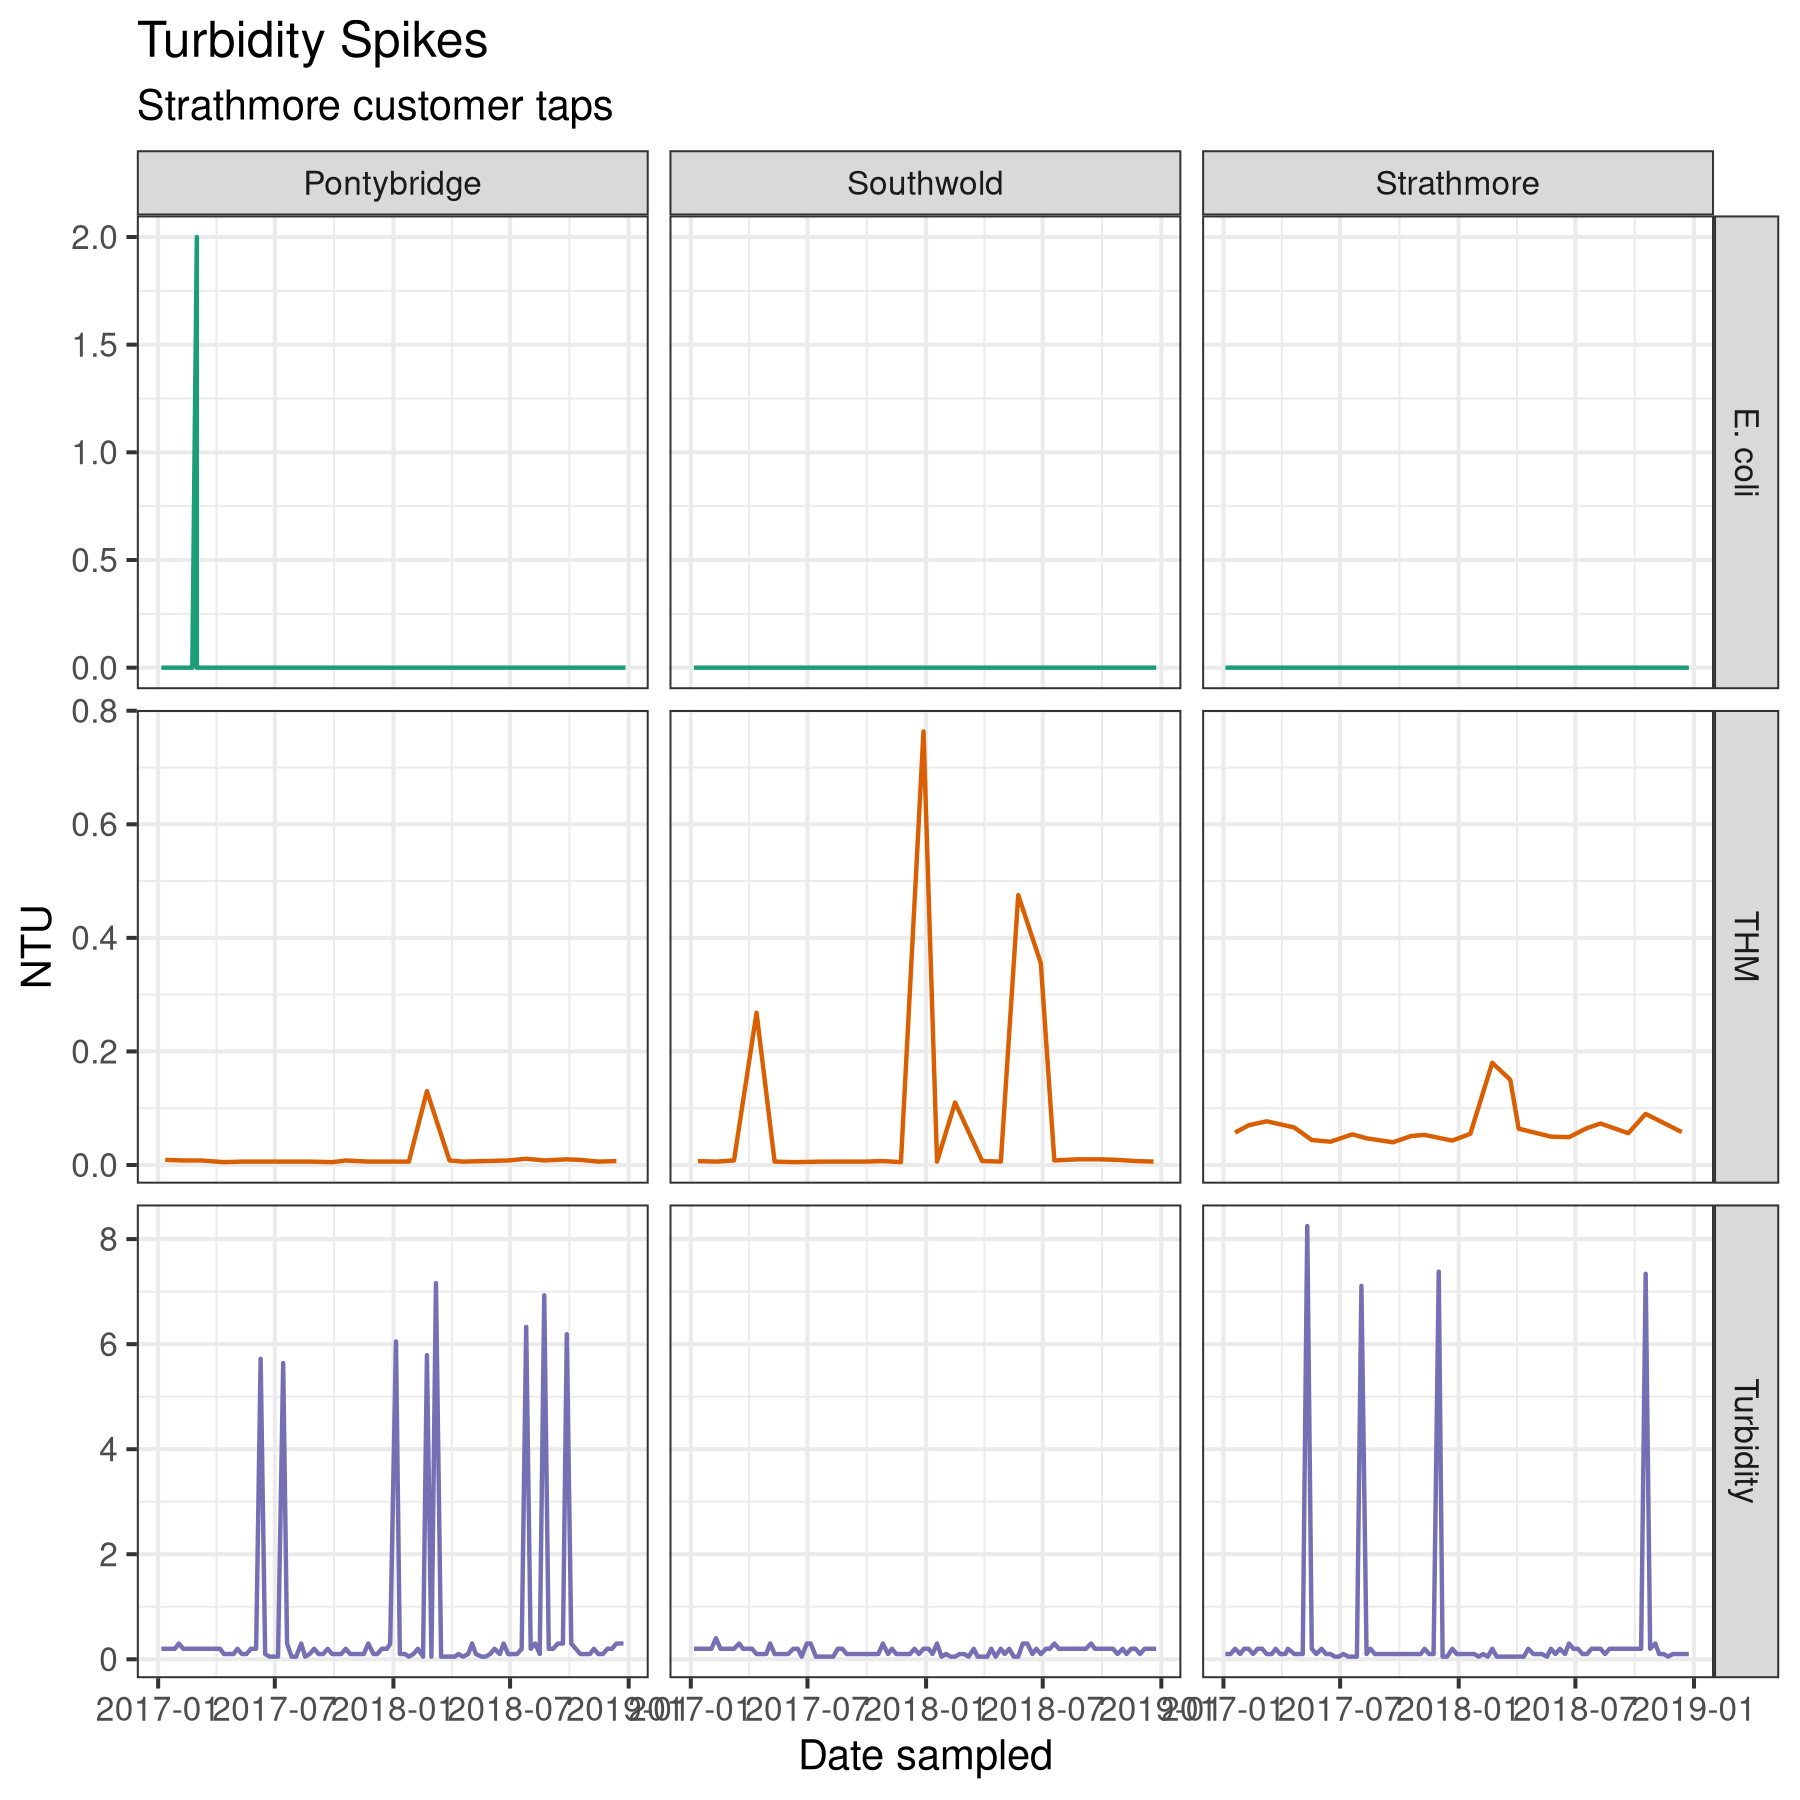
\includegraphics{images/ggplot.png}
\caption{ggplot2 Example}
\end{figure}
\end{column}
\end{columns}
\end{frame}

\begin{frame}{Visualisation Exercise}
\protect\hypertarget{visualisation-exercise}{}
\begin{columns}[T]
\begin{column}{0.48\textwidth}
Use your knowledge of the Gormsey data to create two visual data
stories. Use the following four steps:

\begin{enumerate}
\tightlist
\item
  Explore the data and define the story you want to tell.
\item
  Decide on the best way to visualise the story.
\item
  Develop the basic visualisation.
\item
  Select a theme and annotate the graph.
\end{enumerate}
\end{column}

\begin{column}{0.48\textwidth}
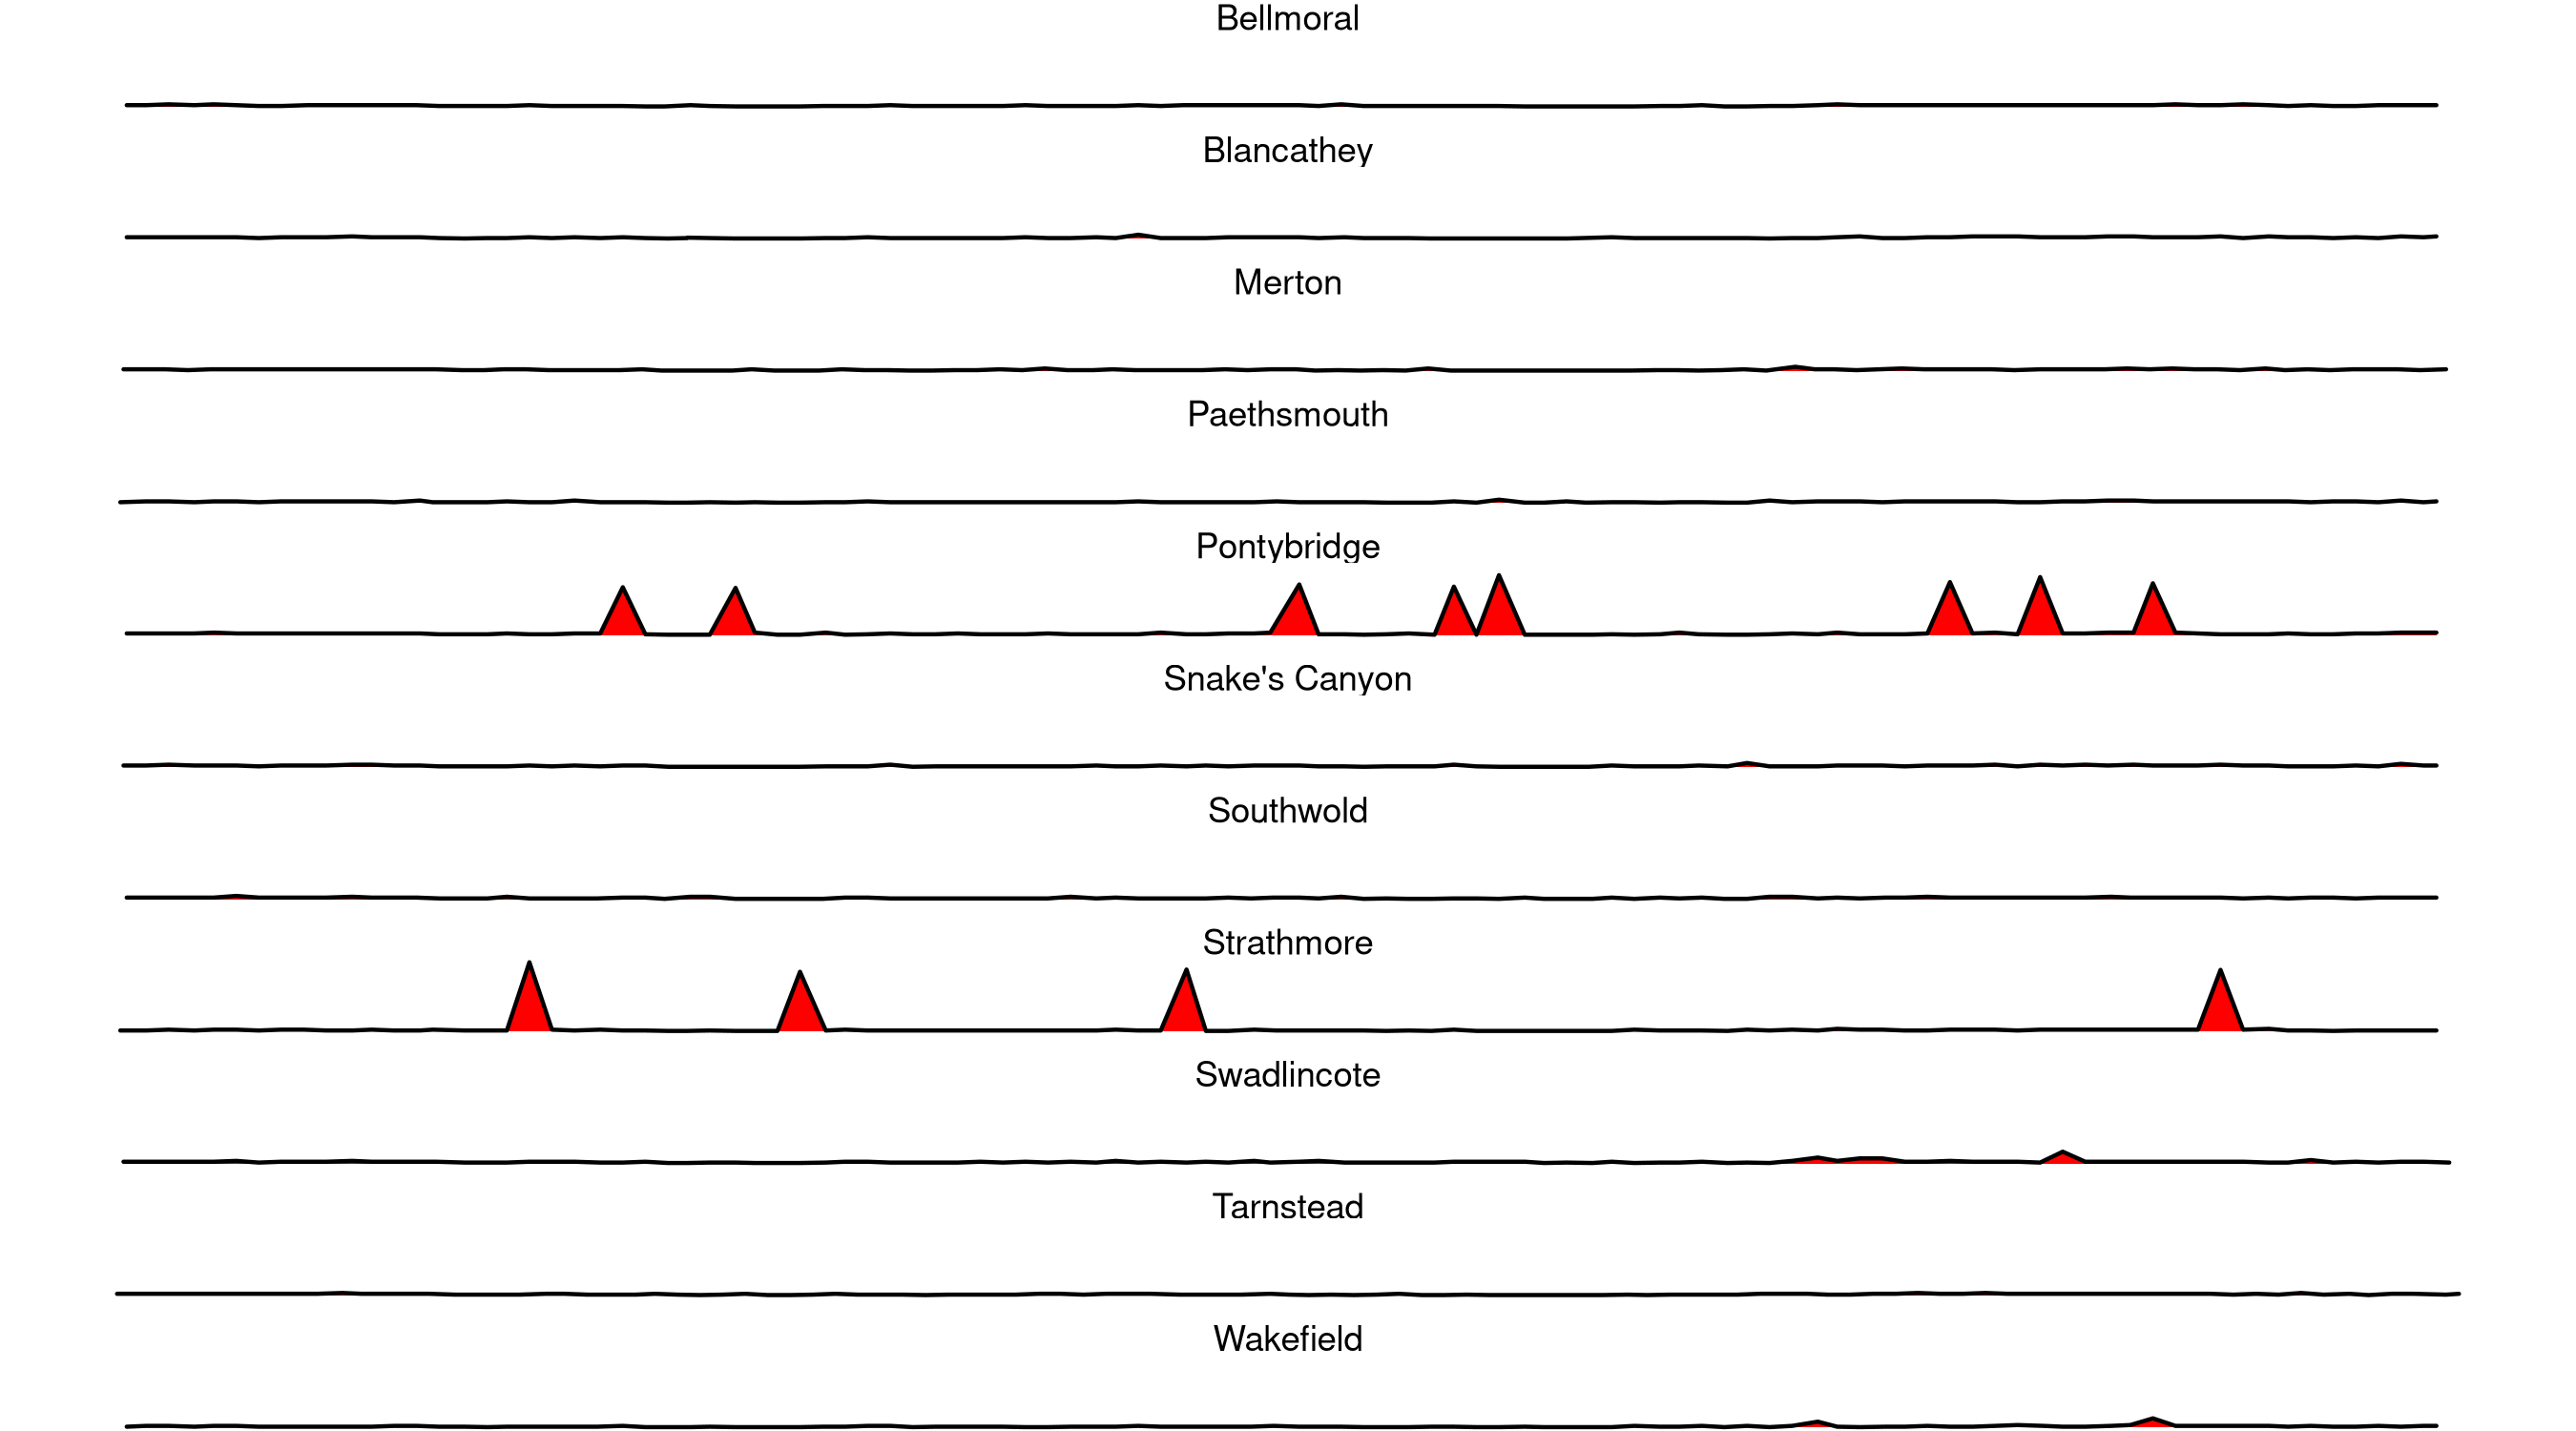
\includegraphics{../manuscript/resources/06_visualisation/sparklets.png}
\end{column}
\end{columns}
\end{frame}

\begin{frame}{Data Science Workflow}
\protect\hypertarget{data-science-workflow}{}
\begin{figure}
\centering
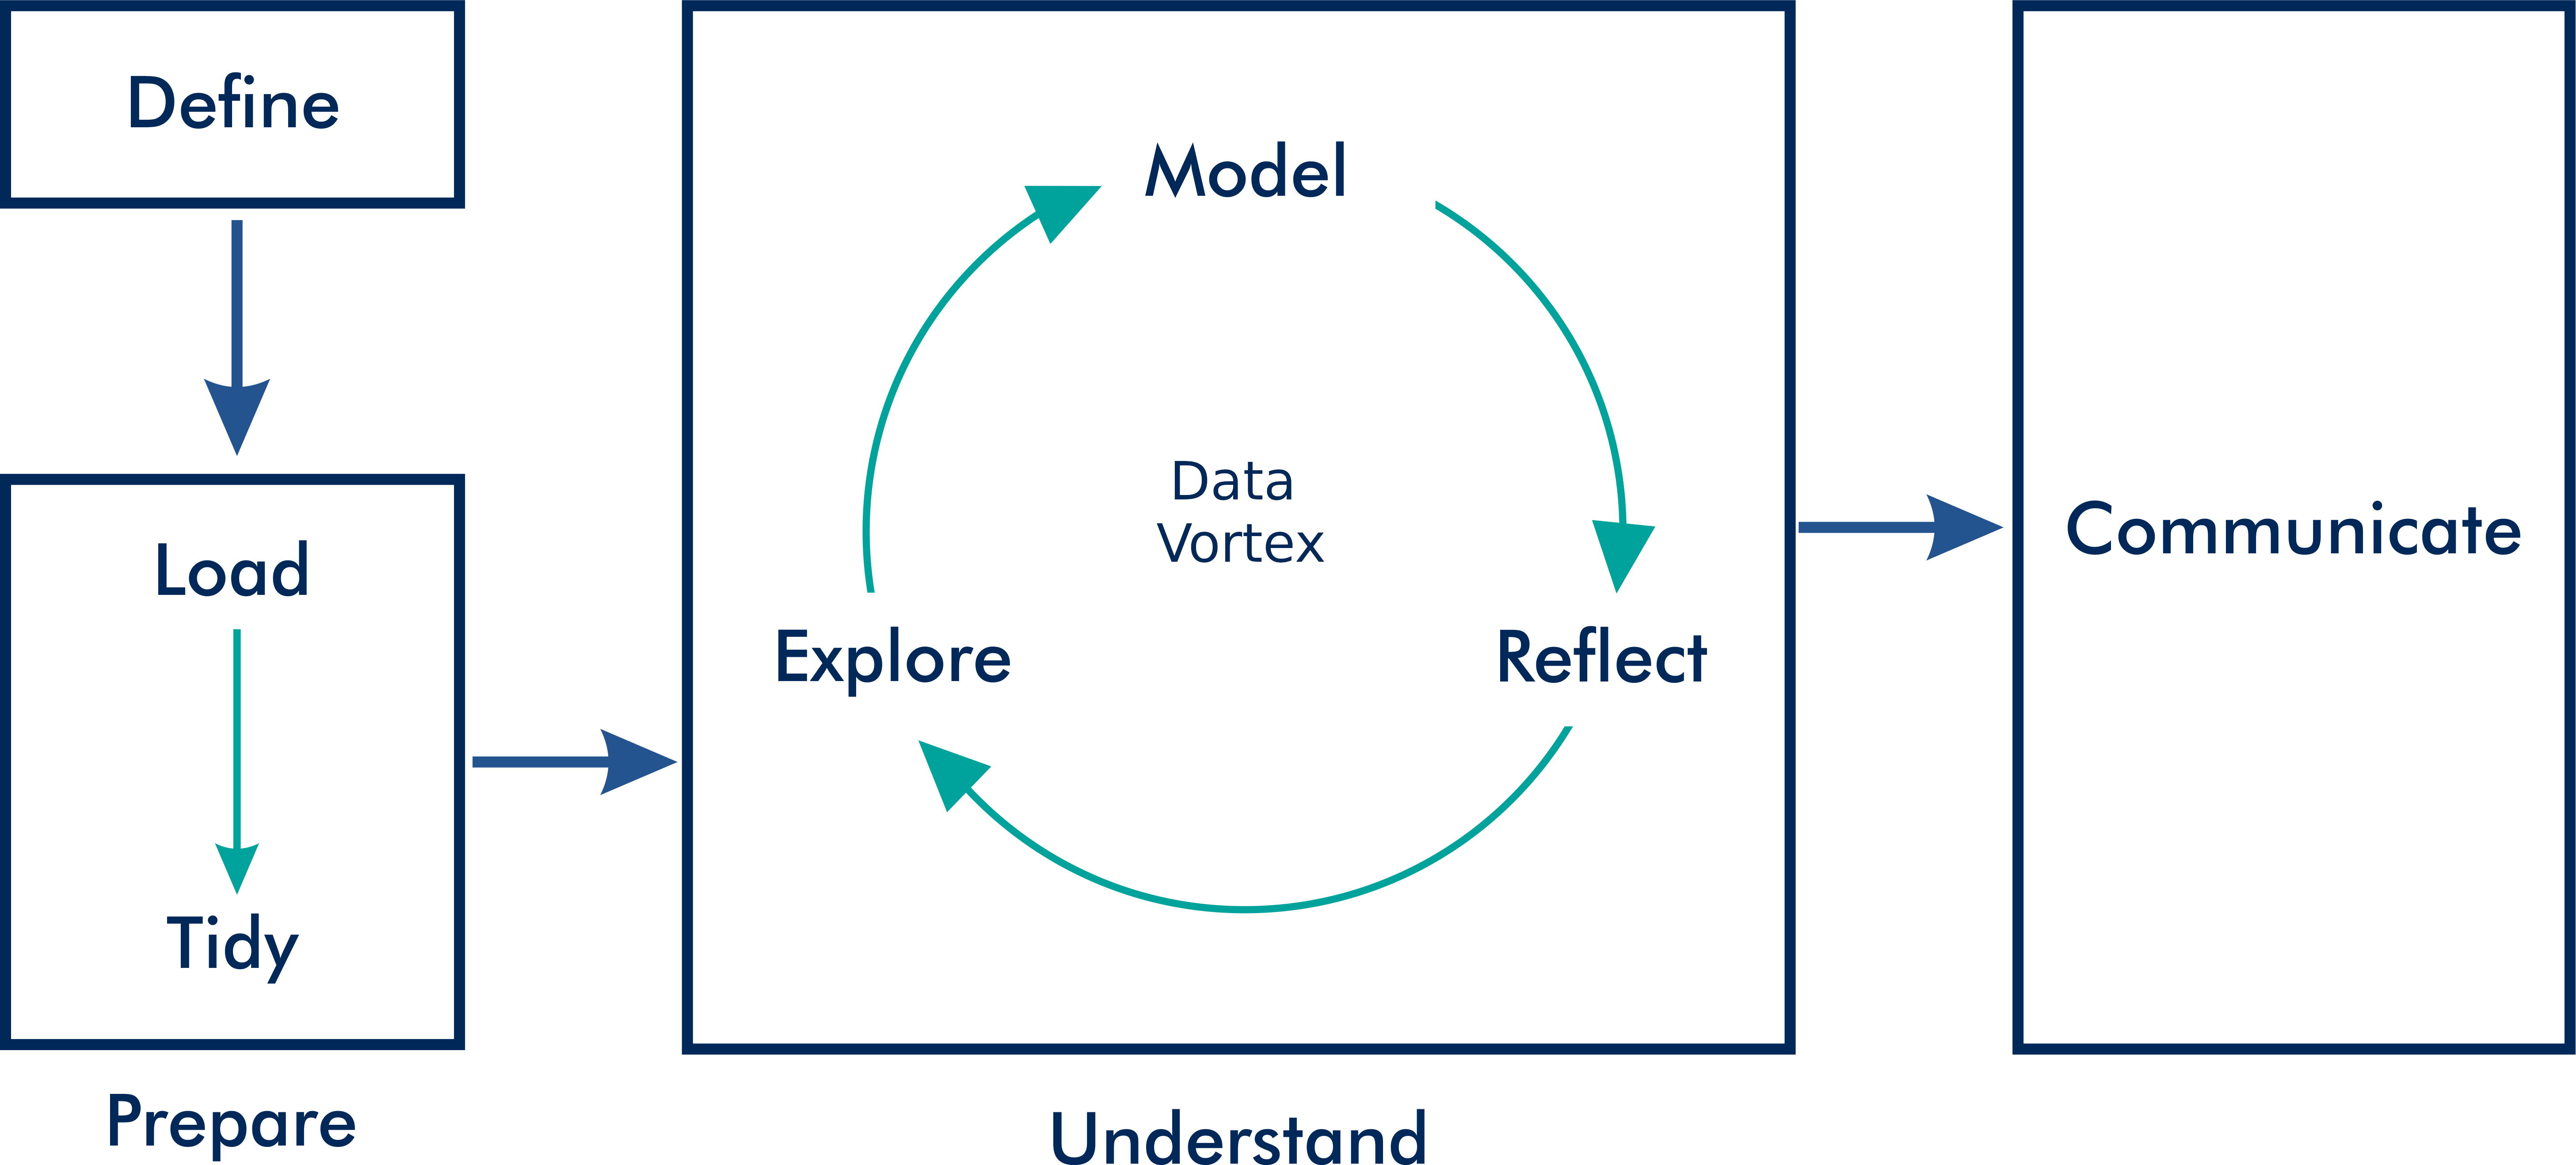
\includegraphics{../manuscript/resources/07_data_products/workflow.png}
\caption{Data science wokflow}
\end{figure}
\end{frame}

\begin{frame}{Data Products}
\protect\hypertarget{data-products}{}
\begin{columns}[T]
\begin{column}{0.48\textwidth}
Static

\begin{itemize}
\tightlist
\item
  Word documents
\item
  PowerPoint presentaions
\item
  Web pages
\end{itemize}

Dynamic

\begin{itemize}
\tightlist
\item
  Shiny application
\item
  Shiny presentation
\end{itemize}

Share - RStudio Connect - Your own server
\end{column}

\begin{column}{0.48\textwidth}
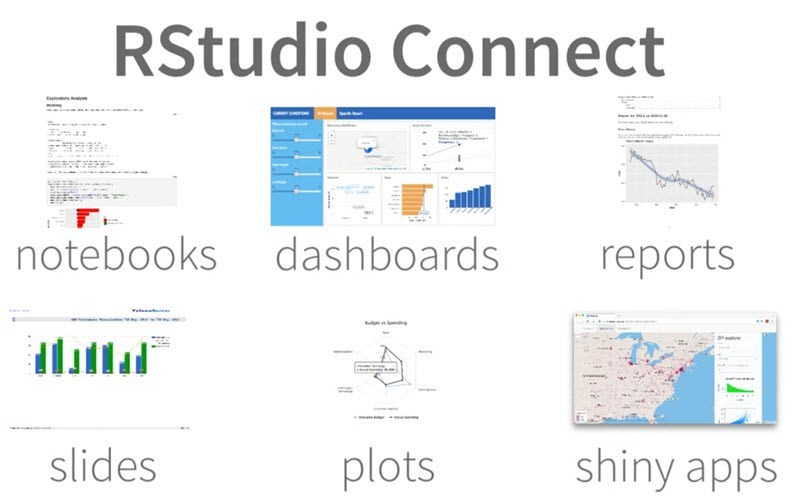
\includegraphics{images/rstudio_connect.jpg}
\end{column}
\end{columns}
\end{frame}

\begin{frame}{RMarkdown}
\protect\hypertarget{rmarkdown}{}
\begin{columns}[T]
\begin{column}{0.48\textwidth}
Literate programming:

\begin{itemize}
\tightlist
\item
  Combine prose with code
\item
  Link the code to dynamic data
\item
  Generate shareable output from code
\end{itemize}
\end{column}

\begin{column}{0.48\textwidth}
Data products:

\begin{itemize}
\tightlist
\item
  Reports
\item
  Web sites
\item
  Presentations
\item
  Applications (dashboards)
\end{itemize}
\end{column}
\end{columns}
\end{frame}

\begin{frame}{RMarkdown Syntax}
\protect\hypertarget{rmarkdown-syntax}{}
\begin{figure}
\centering
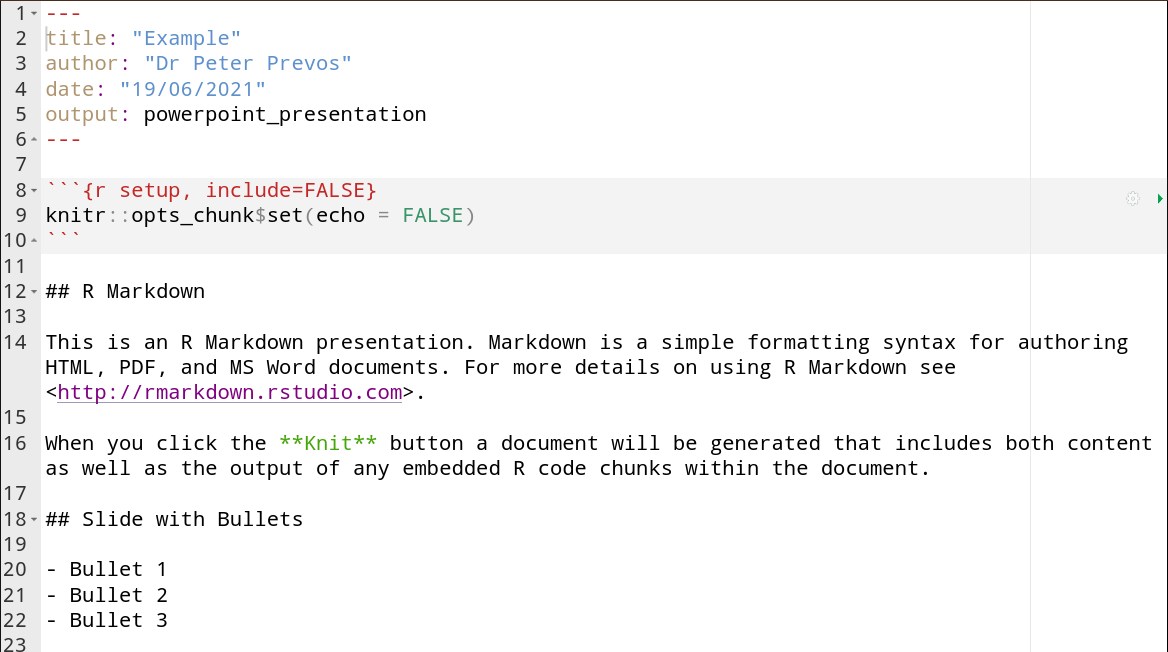
\includegraphics{../manuscript/resources/07_data_products/rmarkdown-example.png}
\caption{RMarkdown syntax example}
\end{figure}
\end{frame}

\begin{frame}[fragile]{Finding Help}
\protect\hypertarget{finding-help}{}
\begin{columns}[T]
\begin{column}{0.5\textwidth}
\begin{itemize}
\tightlist
\item
  Built-in \texttt{help()} function
\item
  Cheat sheets (RStudio and Tidyverse websites)
\item
  Use the R4H2O Slack channel
\item
  Twitter \#rstats
\item
  Reddit rstats, rlanguage
\item
  stackoverflow.com
\item
  Google the problem
\end{itemize}
\end{column}

\begin{column}{0.5\textwidth}
\begin{figure}
\centering
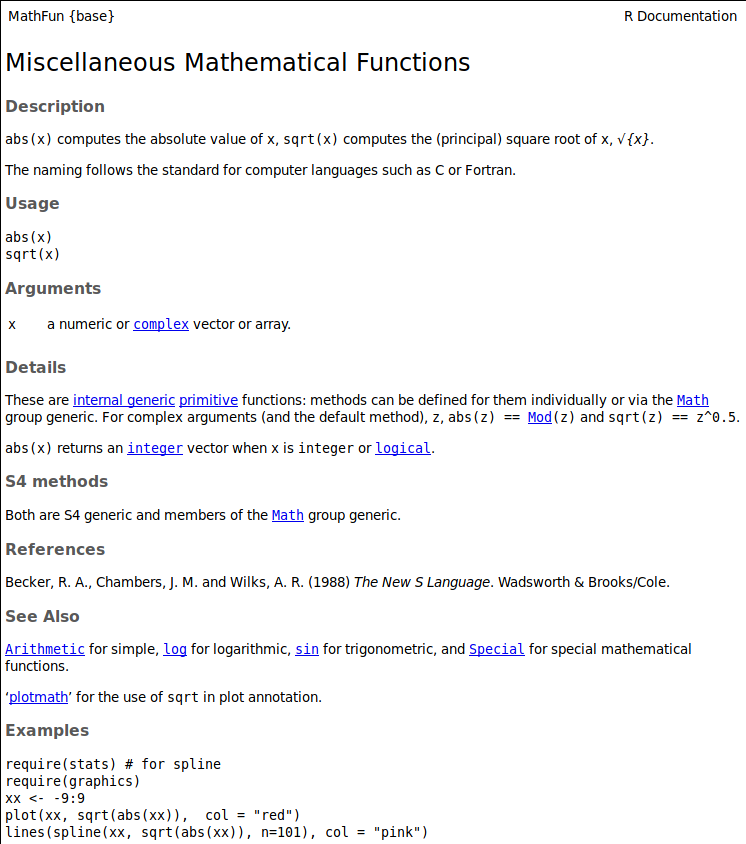
\includegraphics{images/help.png}
\caption{screenshot of help window.}
\end{figure}
\end{column}
\end{columns}
\end{frame}

\begin{frame}{Mini Hackathon}
\protect\hypertarget{mini-hackathon}{}
To close this day, we will do a mini hackathon.

\begin{enumerate}
\tightlist
\item
  Create a script that results in a PowerPoint presentation about the
  Gormsey data.
\item
  Pick a story you like to tell about this data.
\item
  Create a RMarkdown script that results in a Powerpoint presentation.

  \begin{itemize}
  \tightlist
  \item
    Add an introduction.
  \item
    Explore the data.
  \item
    Share the story.
  \end{itemize}
\end{enumerate}
\end{frame}

\end{document}
